\section{Introduction}
Machine-to-Machine communication (M2M), also known as Machine Type Communication (MTC), is an emerging technology allowing devices to mutually communicate without (or only limited) human intervention, which is expected to gain a more popularity in the next decade and be an integrated part of future wireless networks~\cite{3GPP/service-requirement}\cite{3GPP/ranimprovements}. As an example, Ericsson estimates that $2$ out of $50$ billion MTC devices in $2020$ will be connected by cellular technology~\cite{Eri11}. 

MTC presents lots of its own characteristics different from traditional Human-to-Human (H2H) or Human Type Communication (HTC) : uplink-centric applications, short but more frequent transmission, large number of devices, difficulty to change battery and so on \cite{FirstLook12}. Therefore, to well accommodate MTC traffic in the future wireless networks, two possible approaches are envisaged: \begin{itemize}[leftmargin=*, noitemsep]
	\item Design from scratch of M2M-dedicated networks, i.e., the emerging Low Power Wide Area Network (LPWAN). A representative example is the LoRaWAN~\cite{lora/specification} proposed by LoRa Alliance~\cite{lora_alliance};
	\item Evolution from existing wireless networks, which consists in adapting 3GPP cellular networks to support MTC traffic apart from HTC traffic, for example the LTE-M~\cite{ratasuk2014narrowband}.
\end{itemize}
Cisco estimates that the LPWA  and evolved 3GPP networks will have a dominant role for handling MTC traffic in future. It is expected that $29\%$ of MTC devices will be served by LPWA networks and $77\%$ of M2M connections will be served by 3GPP networks (including 2G/3G/4G, shown in Fig.~\ref{fig:m2m-evolution-trend}). The reason relies in that 3GPP cellular networks, compared with LPWA networks, have ubiquitous coverage, largely deployed infrastructure, mature user subscription/management system and so on. 
%\begin{figure}[h]
%	\centering
%	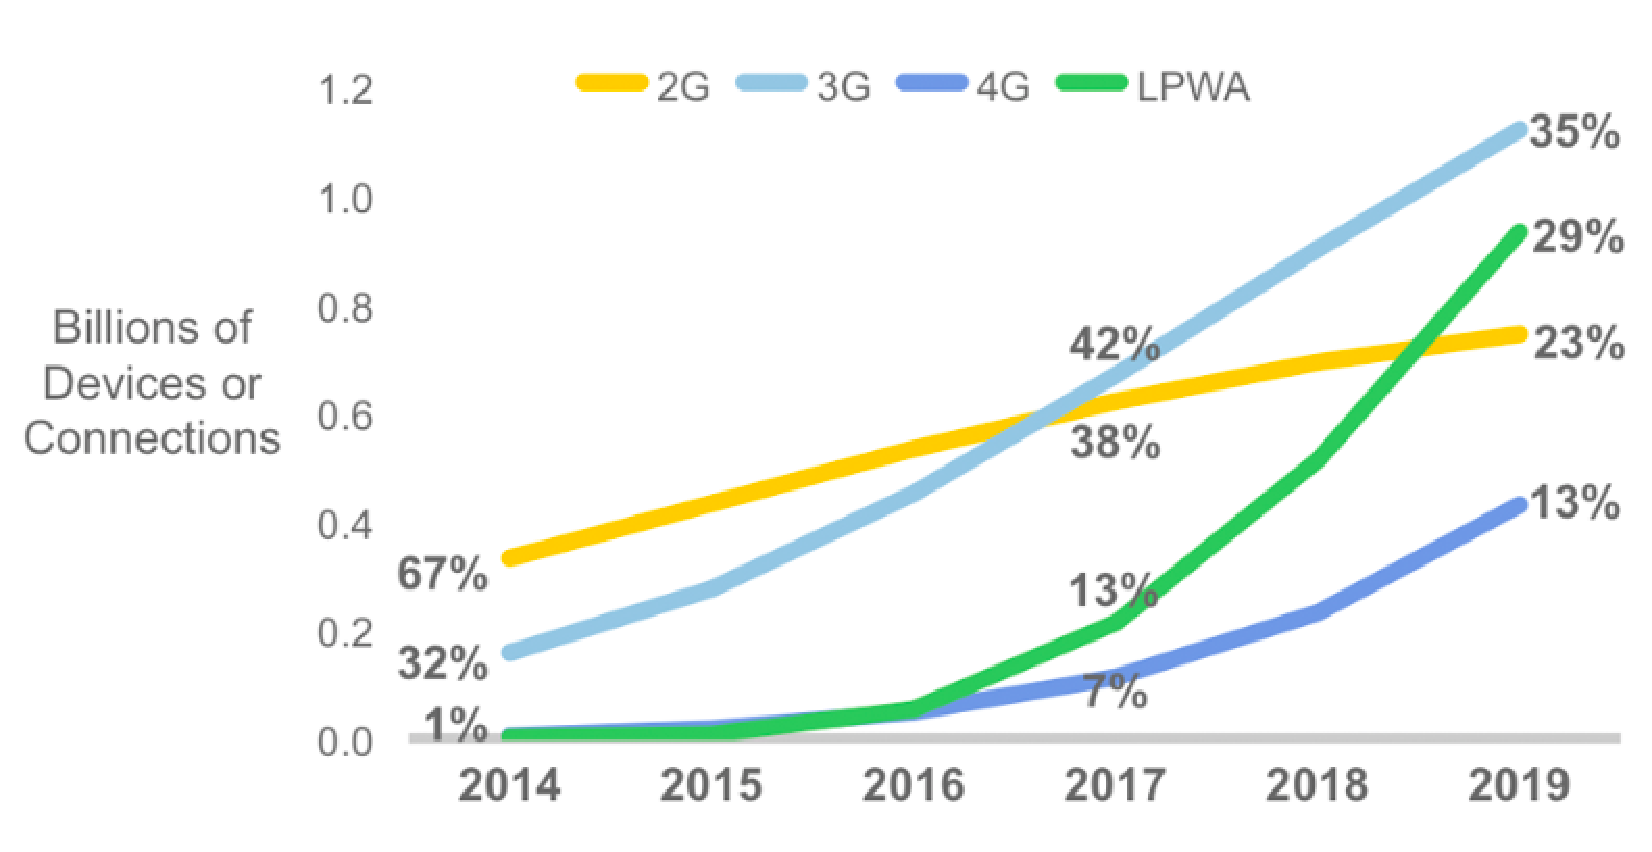
\includegraphics[width=0.9\linewidth, height=4cm]{Chapter2/Figures/Global-mobile-m2m-connections-share}
%	\caption{\csentence{Global M2M growth and migration from 2G to 3G and 4G}. Source: \cite{cisco2015forecast}}
%	\label{fig:m2m-evolution-trend}
%\end{figure}

For both aforementioned approaches, the challenges to be solved are the same: MTC subscription, network/overload control (also called massive access control), security in M2M, diverse QoS provisioning, energy efficiency, etc. Recently the energy efficiency related research has attracted more and more attention, since it is deemed as a key performance indicator that determines if MTC is accepted as a promising technology~\cite{lu11GRS}\cite{Costa14}. Note that the energy efficiency actually covers device side and network side. For cellular M2M, the network side energy efficiency~\cite{suarez2012overview}\cite{wang2014voting} is not a principal constraint, hence it is not within the scope of this article. Instead, MTC devices are usually battery-operated, transmit small data and require a long battery lifetime~\cite{YuanHo12}. The device side energy efficiency is a key problem to make 3GPP cellular networks as a competitive solution for MTC. Thus, we put more focus on research advance about the cellular MTC energy efficiency issue, especially in radio access networks.

%To address the difficulties for well supporting cellular MTC, the Standardization Developing Organizations (SDO) have launched their activities in their own fields. The dominant players in M2M landscape are ETSI M2M and 3GPP LTE. 3GPP has recently become very active in M2M landscape. The focus of 3GPP is the improvement of radio access and core network to facilitate MTC over 3GPP networks. The first 3GPP report related to M2M~\cite{3GPP/TR/facilitating} issued in 2007 indicates a huge market potential for M2M beyond the current market segment. During the age of 3G, there have been little developments about MTC, since CDMA-based 3G systems are not suitable for low power operations. With the emergence of OFDM-based LTE, cellular M2M has become of interest and a set of further documents has been issued. MTC features and service requirements are defined in~\cite{3GPP/service-requirement}. An architectural reference model for MTC, key issues and possible solutions, are presented in~\cite{3GPP/TR/23888V11}.
%%The contribution of Release 11 with regard to MTC... Release 12: Study network improvements for MTC device to MTC device communications via one or more PLMNs (direct-mode communication between devices is out of scope), etc. 
%Recently, 3GPP also study to introduce a new class of User Equipment (UE) with low-cost feature in Release 13~\cite{3GPP/low-cost-device}.
%In addition, 3GPP also aligns with ETSI Technical Committee M2M work.
%ETSI M2M is composed by various manufacturers, operators and service providers, among others. To enable interoperability between M2M services and networks, ETSI established a Technical Committee (TC) in 2009 focusing on M2M service level and defined a M2M reference architecture and interfaces specification~\cite{ETSI/TS/102/690}.
%
%%M2M-related Projects in industrial field
%Besides, there are some international projects for facilitating MTC over 3GPP cellular networks. The EXALTED project (Expanding LTE for Devices, 2010-2013)~\cite{EXALTED}, a Europe FP7 project, is one of the flagship projects in M2M landscape. The main goal of this project is to develop a cost-, spectrum-, and energy-efficient radio access technology for M2M applications, the so-called LTE-M overlay, adapted to coexist within a high-capacity LTE network. Special attention was paid to scalability issues (to, e.g., avoid congestion in the random access procedures) and cost aspects, to ensure affordability of LTE M2M modules. 
%Within this project, a lot of specific issues related to M2M communication in cellular network are studied, including radio resource allocation, relaying, security, PHYsical Layer, coding, emergency and rescue networks along with important standardization activity~\cite{bartoli2011low}\cite{GotsisLA12}. 
%The METIS (Mobile and Wireless Communications Enablers for the Twenty-Twenty Information Society) is a Europe FP7 project from 2012 to 2015. Its global objective is to lay the foundation for the 5G system. With regard to MTC, they focus how to efficiently support Massive Machine-Type Communication (mMTC) and Utra-reliable Machine-Type Communication (uMTC) in the future 5G, by studying technologies about radio Links, multi-node/multi-antenna transmission and so on.
%LOLA (Achieving Low-Latency in Wireless Communications) \cite{lola} project focuses on physical and MAC layer techniques aimed at achieving low-latency transmission in cellular (LTE and LTE-A) and wireless mesh networks.

With regard to cellular M2M related surveys, Taleb et al.~\cite{journals/cm/TalebK12} focus MTC devices subscription control and network congestion/overload control. Chen et al.~\cite{chen2014machine} talk research efforts for efficient MTC and explore various M2M-related issues such as deployment, operation, security and privacy. Andres et al.~\cite{laya14} make a survey of proposals improving the operation of random access channel of LTE/LTE-A and evaluate the energy consumption of LTE RACH procedure. Poncela et al. \cite{poncela2015m2m} identify the limitations of 4G for MTC (signaling, scheduler) and resume the improvements of LTE/LTE-A to handle M2M traffic. Several review papers~\cite{GhavimiF2015}\cite{mehmood2015mobile} discuss MTC in 3GPP LTE/LTE-A networks, introduce M2M uses cases in detail and identify the challenges with regard to M2M over LTE/LTE-A, e.g., random access congestion, resource allocation with QoS provisioning. Wang et al.~\cite{wang2012survey} survey and discuss various remarkable techniques, in terms of all components of the mobile networks (e.g., data centers, marcocell, femtocell, etc.), toward green mobile cellular networks. Ismail et al.~\cite{ismail2014survey} investigate the energy-efficiency from perspective of network operators and mobile users. Yang et al.~\cite{yang2015software} make a survey about software-defined wireless network (SDWN) and wireless network virtualization (WNV) for the future mobile wireless networks, which help define the future mobile wireless network architecture to tackle with heterogeneous traffic.

To our best knowledge, a comprehensive survey about device side energy efficiency issues in radio networks used for cellular M2M service is still not available in the literature. Therefore, the goal of this article is to compare and categorize existing M2M-related energy efficiency proposals before discussing the trends for cellular M2M research. In addition, in this article we want to provide a short overview of cellular M2M applications, detail different types of classification of M2M services and propose a synthesis for the QoS demands. We also review the advances of Low Power Wide Area networks, which are MTC-dedicated networks, and today are experiencing a rapid development. The rest of this article is organized as follows. Section~\ref{sec:m2m-app-class} presents the typical cellular M2M applications and several classifications according to different criteria, introduces a QoS requirement table for some typical cellular M2M applications. Section~\ref{sec:diff-traffic} compares the differences between H2H and M2M in terms of traffic characteristics. Section~\ref{sec:ref-m2m-arch} first talks about conventional M2M solutions in cellular networks then presents the advance of reference M2M network architecture. Section~\ref{sec:lpwa} resumes the development of Low Power Wide Area networks. Section~\ref{sec:proposals} presents, categorizes and compares all found proposals related to energy issues for MTC in cellular networks. Section~\ref{sec:conclusion} gives the conclusions obtained from this survey.